\documentclass[crop, tikz]{standalone}
\usepackage{tikz}

\usetikzlibrary{arrows,shapes, decorations.pathmorphing,backgrounds,positioning}
\usetikzlibrary{decorations.pathreplacing}
\usetikzlibrary{arrows.meta}

\tikzstyle{smallnode}=[draw, circle, inner sep=2pt]
\tikzstyle{stateTransition}=[->, thick, -{Latex[length=2mm,width=2mm]}]


\begin{document}
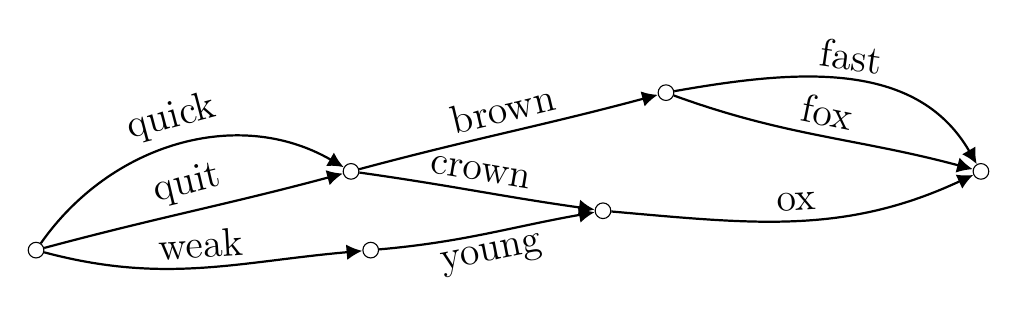
\begin{tikzpicture}
    \node[smallnode] (n1) at (0, 0) {};
    \node[smallnode] (n2) at (0.25, -1) {};
    
    \node[smallnode] (n3) at (4, 1) {};
    \node[smallnode] (n4) at (3.2, -0.5) {};

    \node[smallnode] (n5) at (8, 0) {};
    \node[smallnode] (n6) at (-4, -1) {};
    
    % Arcs
    \draw[stateTransition] (n6) to[out=15,in=195] node [midway, sloped, above] {\Large{quit}} (n1);
    \draw[stateTransition] (n6) to[out=55,in=150] node [midway, sloped, above] {\Large{quick}} (n1);
    \draw[stateTransition] (n6) to[out=-15,in=185] node [midway, sloped, above] {\Large{weak}} (n2);
    
    \draw[stateTransition] (n1) to[out=352,in=172] node [midway, sloped, above] {\Large{crown}} (n4);
    
    \draw[stateTransition] (n3) to[out=-20,in=165] node [midway, sloped, above] {\Large{fox}} (n5);
    \draw[stateTransition] (n4) to[out=-5,in=205] node [midway, sloped, above] {\Large{ox}} (n5);
    \draw[stateTransition] (n3) to[out=10,in=120] node [midway, sloped, above] {\Large{fast}} (n5);
    
    \draw[stateTransition] (n1) to[out=15,in=195] node [midway, sloped, above] {\Large{brown}} (n3);
    \draw[stateTransition] (n2) to[out=5,in=190] node [midway, sloped, below] {\Large{young}} (n4);

\end{tikzpicture}

\end{document}